% sage_latex_guidelines.tex V1.20, 14 January 2017

% 4000-6000 words, 2000 here as of everything but results and conclusion complete

\documentclass[sagev,times,Royal]{sagej}
% add 'doublespace'

\usepackage{moreverb,url}

\usepackage{graphicx}

\usepackage[colorlinks,bookmarksopen,bookmarksnumbered,citecolor=red,urlcolor=red]{hyperref}

\newcommand\BibTeX{{\rmfamily B\kern-.05em \textsc{i\kern-.025em b}\kern-.08em
T\kern-.1667em\lower.7ex\hbox{E}\kern-.125emX}}

\def\volumeyear{2021}

\begin{document}

\runninghead{Pape}

\title{Energy simulation and analysis of accessory dwelling units: 
an evolutionary approach}

\author{P. Arthur Pape\affilnum{1}}

\affiliation{\affilnum{1}University of Washington}

\corrauth{P. Arthur Pape}

\email{ppape@uw.edu}

\begin{abstract}
Accessory dwelling units (ADUs) are surging in popularity as cities push for their construction to aid in combatting the housing crisis. In Seattle, Washington, recent survey data calls for increased focus on sustainability and cost. Lowering energy use intensity (EUI) of ADUs allows for the targeting of both desires which homeowners hold. The effect of varying window-to-wall ratios (WWRs) on EUI is simulated using EnergyPlus and Honeybee. Galapagos, a genetic solver plugin for Grasshopper is used to vary window-to-wall ratio and optimize ADU energy use intensity on three single family residential lots in Seattle. Site context is constructed using OpenStreetMap GIS data and zoning restrictions are incorporated into the Grasshopper definition. Future work is planned to utilize output data from this tool as the training dataset for a machine learning model. Accurate machine learning prediction of energy use intensity instead of extended simulation would increase pragmatic use of such tools.
\end{abstract}

\keywords{Genetic algorithm, accessory dwelling unit, housing, optimization, simulation, energy use intensity, grasshopper, galapagos}

\maketitle

\section{Introduction}
The United States is amidst an unprecedented housing crisis, stemming from parallel crises: from neoliberal austerity spending cuts towards social benefits to the near-virtual lack of social housing and rent control programs in the United States to the ever-increasing privatization of essentially every aspect of American life\cite{10.2307/26297969}. The result is a rising population of unhoused peoples and the inability for many to become a homeowner or to even afford minimum monthly rent in many cities. Solutions to this dilemma are neither straightforward nor definite. However, designers and architects can only address the symptom-level problems, while advocating towards change directed at the root cause. 

Seattle, Washington; Portland, Oregon; and Vancouver, British Columbia are exploring the use of accessory dwelling units (ADUs) as one method to combat surging housing prices. Use of ADUs is an effective means of increasing housing density without replacing single family (SF) housing zones with new multi family residential construction. Additionally, ADUs are often designed to be rented, generating supplementary income for the homeowner. Historically, homeowner’s associations and other local organizations have  been resistant to any proposed density increases through zoning or other means\cite{10.2307/24392672}. However, Seattle and the other previously mentioned cities in the Pacific Northwest have succeeded in allowing for the construction of ADUs in recent decades, with these groups beginning to see ADUs as a positive. ADUs offer many positives beyond an increased housing supply such as a path for homeowners to generate income and accommodating households with multigenerational or caretaking needs.

Beginning in 2014, the City of Seattle has moved to increase production of ADUs through various resolutions and legislation, in turn removing barriers to entry and highlighting strategies for encouragement. In late 2019, a call for detached ADU (or DADU) designs was issued to designers. As a result, ten DADU designs were pre-approved by the City of Seattle and are available online to entice homeowners\cite{ADUniversePreapprovedADU}. The pre-approved designs are free, but still require standard permitting fees to be paid for approval and come with one significant downside of many other pre-designed structures: a lack of contextual design and individualization. This one-size-fits-all approach can have drastic effects upon energy consumption, reducing the appeal of such an investment. Further, these designs do not offer the scalability or energy efficiency that an ADU designed specifically per site offers.

 Coincidentally, a November 2019 city survey shows that there are calls for an increased focus on sustainability and cost in the construction of ADUs\cite{seattlePreapprovedPlansAccessory2019}. This survey was positioned before the official call for submissions was broadcast. 'Low cost' was the top ranked criteria with 48\% of responses listing 'very important', followed by 'green building' being ranked similarly at 46\%. Other suggestions sourced from surveyed respondents included low environmental costs, site specific considerations, and predictability. The ability to show users the estimated annual energy consumption of a new construction DADU would have a major impact on driving construction demand based on survey responses noted. Using an optimization method such as a genetic algorithm (GA) can allow architects to arrive at the most effective design solution on a site specific basis while predictably minimizing both environmental and financial costs. 
 
\section{Methodology} 
This research explores the use of a genetic solver to find the optimal design solution of window-to-wall ratios (WWR) for a simple DADU form resulting in the lowest energy use intensity (EUI) value. Three sites in comparable neighborhoods in the city of Seattle were selected based on a combination of proximity and slight density variance. The tool adheres to zoning regulations to find estimated buildable area for a DADU on each site, creates a simple box-like form representing the DADU and then varies the WWR value for each of the four walls. A genetic solver plugin is then allowed to vary these ratios to find an optimal solution using a process largely mimicking natural genetic processes. Finally, an energy model is created from each individual iteration to find an estimate for overall EUI. From here, the process loops until an optimal solution is found.

Site locations were chosen through the use of the ADUniverse tool, developed by University of Washington researchers at the eScience Institute's \textit{Data Science for Social Good} program\cite{ADUniverseToolEScience}. ADUniverse allows for users to investigate the possibility of constructing an ADU through a map-based user interface. Chosen sites are located within the Madrona, Minor, and Central District neighborhoods of Seattle, WA. All three sites are zoned under SF5000, a single family residential zoning. Site data was extracted from open source map website OpenStreetMap.org and converted into an AutoCAD .DWG file. Next, this 2D linework was imported into and extruded into three dimensions within Rhinoceros 6 (Rhino) and Grasshopper, a 3D modeling software and visual scripting tool for Rhino, respectively. Property lines (pulled from the Seattle City GIS tool) for each chosen residential site are fed into the Grasshopper definition, coupled with constraints in-line with the current land use code of Seattle \cite{SeattleLandUse2021}. Such universal constraints for ADUs on lots located within SF5000 zoning are as follows\cite{ADUniverseADURules}: 

% Itemized list of zoning restrictions for each site
\begin{itemize}
	\item Lot size must be at least 3200 square feet
	\item Minimum lot width of 25 feet
	\item Minimum lot length of 70 feet
	\item DADU can occupy \textit{at most} 60\% of rear yard	
	\item Front yard of 20 feet, side yards of 5 feet, rear yard of 25  feet
	\item DADU height limit varies based on lot width: \begin{itemize}
	\item 14 feet for lot widths less than 30 feet
	\item 16 feet for lot widths between 40 and 50 feet
	\item 18 feet for lot widths exceeding 50 feet \end{itemize}
\label{zoning-restrictions}
\end{itemize}

These constraints are built into the Grasshopper definition in such a way that the tool requires simply lot extents and the footprint of the existing residential structure to develop the buildable area for any DADU construction. Each DADU is represented as a simple 12' shoebox model with facades oriented  perpendicular to the cardinal directions. Under current Seattle Residential Building Code (2018), minimum R-values for wall and ceiling assemblies are R-21 and R-49, respectively. Light wood frame construction was chosen for all three sites, as the majority of residential construction in the United States and in Seattle specifically falls under this category due to price and ubiquity. For this project, total R-values were set to 26.86, 54.592, and 5.73, for wall, roof, and floor assemblies, respectively. Wall and roof assemblies are detailed in Tables \ref{table:wall-assembly} and \ref{table:roof-assembly}. Floor condition is a standard slab-on-grade with rigid insulation below an 8" concrete slab, finished with carpeting.

% Wall Assembly
\begin{table}[]
\centering
\resizebox{\textwidth}{!}{%
\begin{tabular}{lcccc}
\hline
\multicolumn{1}{|l|}{\textbf{Assembly}} &
  \multicolumn{1}{l|}{\textbf{Notes}} &
  \multicolumn{1}{c|}{\textbf{R-Value}} &
  \multicolumn{1}{l|}{\textbf{Path 1 (Insulation)}} &
  \multicolumn{1}{l|}{\textbf{Path 2 (Framing)}} \\ \hline
\multicolumn{1}{|l|}{Air Film} &
  \multicolumn{1}{c|}{Interior} &
  \multicolumn{1}{c|}{0.68} &
  \multicolumn{1}{c|}{0.68} &
  \multicolumn{1}{c|}{0.68} \\ \hline
\multicolumn{1}{|l|}{Gypsum Board} &
  \multicolumn{1}{c|}{1/2"} &
  \multicolumn{1}{c|}{0.45} &
  \multicolumn{1}{c|}{0.45} &
  \multicolumn{1}{c|}{0.45} \\ \hline
\multicolumn{1}{|l|}{Vapor Barrier} &
  \multicolumn{1}{c|}{} &
  \multicolumn{1}{c|}{0} &
  \multicolumn{1}{c|}{0} &
  \multicolumn{1}{c|}{0} \\ \hline
\multicolumn{1}{|l|}{Rigid Insulation} &
  \multicolumn{1}{c|}{4"} &
  \multicolumn{1}{c|}{6} &
  \multicolumn{1}{c|}{24} &
  \multicolumn{1}{c|}{-} \\ \hline
\multicolumn{1}{|l|}{2" x 6" Wood Stud} &
  \multicolumn{1}{c|}{16" o.c.} &
  \multicolumn{1}{c|}{12.31} &
  \multicolumn{1}{c|}{-} &
  \multicolumn{1}{c|}{12.31} \\ \hline
\multicolumn{1}{|l|}{Air Gap} &
  \multicolumn{1}{c|}{1"} &
  \multicolumn{1}{c|}{2.38} &
  \multicolumn{1}{c|}{2.38} &
  \multicolumn{1}{c|}{2.38} \\ \hline
\multicolumn{1}{|l|}{Wood Cladding} &
  \multicolumn{1}{c|}{3/4"} &
  \multicolumn{1}{c|}{0.93} &
  \multicolumn{1}{c|}{0.93} &
  \multicolumn{1}{c|}{0.93} \\ \hline
\multicolumn{1}{|l|}{Air Film} &
  \multicolumn{1}{c|}{Exterior} &
  \multicolumn{1}{c|}{0.17} &
  \multicolumn{1}{c|}{0.17} &
  \multicolumn{1}{c|}{0.17} \\ \hline
 &
  \multicolumn{1}{c|}{} &
  \multicolumn{1}{c|}{\textbf{R-Total:}} &
  \multicolumn{1}{c|}{28.61} &
  \multicolumn{1}{c|}{16.92} \\ \cline{3-5} 
 &
  \multicolumn{1}{l}{} &
  \multicolumn{1}{l}{} &
  \textit{x 85\%} &
  \textit{x 15\%} \\
 &
  \multicolumn{1}{l}{} &
  \multicolumn{1}{l}{} &
  24.3185 &
  2.538 \\ \cline{3-5} 
 &
  \multicolumn{1}{l|}{} &
  \multicolumn{1}{c|}{\textbf{Wall R-Value:}} &
  \multicolumn{2}{c|}{26.86} \\ \cline{3-5} 
 &
  \multicolumn{1}{l|}{} &
  \multicolumn{1}{l|}{\textbf{Wall U-Value:}} &
  \multicolumn{2}{c|}{0.0372} \\ \cline{3-5} 
 &
  \multicolumn{1}{l}{} &
  \multicolumn{1}{l}{} &
  \multicolumn{1}{l}{} &
  \multicolumn{1}{l}{}
\end{tabular}%
}
\caption{Wall Assembly}
\label{table:wall-assembly}
\end{table}

% Roof Assembly
\begin{table}[]
\centering
\resizebox{\textwidth}{!}{%
\begin{tabular}{lcccc}
\hline
\multicolumn{1}{|l|}{\textbf{Assembly}} &
  \multicolumn{1}{l|}{\textbf{Notes}} &
  \multicolumn{1}{c|}{\textbf{R-Value}} &
  \multicolumn{1}{l|}{\textbf{Path 1 (Insulation)}} &
  \multicolumn{1}{l|}{\textbf{Path 2 (Framing)}} \\ \hline
\multicolumn{1}{|l|}{Air Film} &
  \multicolumn{1}{c|}{Interior} &
  \multicolumn{1}{c|}{0.61} &
  \multicolumn{1}{c|}{0.61} &
  \multicolumn{1}{c|}{0.61} \\ \hline
\multicolumn{1}{|l|}{Gypsum Board} &
  \multicolumn{1}{c|}{1/2"} &
  \multicolumn{1}{c|}{0.45} &
  \multicolumn{1}{c|}{0.45} &
  \multicolumn{1}{c|}{0.45} \\ \hline
\multicolumn{1}{|l|}{Vapor Barrier} &
  \multicolumn{1}{c|}{} &
  \multicolumn{1}{c|}{0} &
  \multicolumn{1}{c|}{0} &
  \multicolumn{1}{c|}{0} \\ \hline
\multicolumn{1}{|l|}{Cellulose Insulation} &
  \multicolumn{1}{c|}{Blow-in} &
  \multicolumn{1}{c|}{47} &
  \multicolumn{1}{c|}{47} &
  \multicolumn{1}{c|}{-} \\ \hline
\multicolumn{1}{|l|}{2" x 10" Wood Rafters} &
  \multicolumn{1}{c|}{24" o.c.} &
  \multicolumn{1}{c|}{14.68} &
  \multicolumn{1}{c|}{-} &
  \multicolumn{1}{c|}{14.68} \\ \hline
\multicolumn{1}{|l|}{Rigid Insulation} &
  \multicolumn{1}{c|}{2"} &
  \multicolumn{1}{c|}{10} &
  \multicolumn{1}{c|}{10} &
  \multicolumn{1}{c|}{10} \\ \hline
\multicolumn{1}{|l|}{OSB Sheathing} &
  \multicolumn{1}{c|}{7/16"} &
  \multicolumn{1}{c|}{0.77} &
  \multicolumn{1}{c|}{0.77} &
  \multicolumn{1}{c|}{0.77} \\ \hline
\multicolumn{1}{|l|}{Asphalt Shingles} &
  \multicolumn{1}{c|}{} &
  \multicolumn{1}{c|}{0.44} &
  \multicolumn{1}{c|}{0.44} &
  \multicolumn{1}{c|}{0.44} \\ \hline
\multicolumn{1}{|l|}{Air Film} &
  \multicolumn{1}{c|}{Exterior} &
  \multicolumn{1}{c|}{0.17} &
  \multicolumn{1}{c|}{0.17} &
  \multicolumn{1}{c|}{0.17} \\ \hline
 &
  \multicolumn{1}{c|}{} &
  \multicolumn{1}{c|}{\textbf{R-Total:}} &
  \multicolumn{1}{c|}{59.44} &
  \multicolumn{1}{c|}{27.12} \\ \cline{3-5} 
 &
  \multicolumn{1}{l}{} &
  \multicolumn{1}{l}{} &
  \textit{x 85\%} &
  \textit{x 15\%} \\
 &
  \multicolumn{1}{l}{} &
  \multicolumn{1}{l}{} &
  50.524 &
  4.068 \\ \cline{3-5} 
 &
  \multicolumn{1}{l|}{} &
  \multicolumn{1}{c|}{\textbf{Wall R-Value:}} &
  \multicolumn{2}{c|}{54.592} \\ \cline{3-5} 
 &
  \multicolumn{1}{l|}{} &
  \multicolumn{1}{l|}{\textbf{Wall U-Value:}} &
  \multicolumn{2}{c|}{0.0183} \\ \cline{3-5} 
 &
  \multicolumn{1}{l}{} &
  \multicolumn{1}{l}{} &
  \multicolumn{1}{l}{} &
  \multicolumn{1}{l}{}
\end{tabular}%
}
\caption{Roof Assembly}
\label{table:roof-assembly}
\end{table}

\subsection{Energy model and analysis}
Honeybee, part of the open-source Ladybug Tools plugin suite for Grasshopper and Rhino, has become an industry standard for daylighting simulation and energy modeling within architecture and engineering, largely due to its open source nature\cite{mackey2018tool}. Honeybee acts as a bridge between modeled Rhino geometry and the United States Department of Energy's EnergyPlus simulation tool. Modeled geometry is constructed as rooms and zones within Honeybee, offering greater granularity. EnergyPlus operates using various abstractions and simplifications and these are important to note\cite{EnergyPlusTMVersionDocumentation2021}. Each zone and surface is only able to hold one temperature value at a time- each singular value is averaged across the zone or surface. Each DADU simulated is represented as a single zone spanning the entire structure. Alternatively, using four zones and a core instead would have increased resolution of results, but at the cost of much longer simulation times. For building typologies larger than ADUs, this discrepancy between EUI simulation results using one or five (four and a core) zones has been studied\cite{SingleZoneVs2018}. Results showed EUI estimates experienced 4.23\% variance on average for cities tested. Further, for Seattle specifically, results varied by only 2.12\%.
 
Similarly, trees are represented as simple cylindrical solids, in order to keep energy simulation speed quick and to reduce the time necessary to reach an optimal solution. In initial tests, trees were represented as spherical meshes created using Grasshopper. These more-detailed trees varied in opaque triangulated mesh coverage to simulate foliage cover and to more accurately cast shadows. It is important to note that with access to greater computing power it could become reasonable to represent and simulate trees in the original format. Together with other context, including the associated residence and nearby residences capable of projecting shadows onto the DADU, the tree models were assigned as shades in the Honeybee model. 

The final input required for the Honeybee/EnergyPlus model is a weather file, in .EPW (EnergyPlus Weather File) format. These files contain yearly climate data for a geographic location; in this case data was collected at the King County International Airport - Boeing Field in Seattle, Washington. The American Society of Heating, Refrigerating, and Air-Conditioning Engineers (ASHRAE) defines climate zones for use with EnergyPlus and other tools/calculations. Seattle falls within the ASHRAE 169-2006 standard 4C climate, defined as \textit{Mixed - Marine}. This climate type is utilized within the Grasshopper script to define the wood frame construction type for the Seattle climate. EPW files are obtainable freely at \textit{EnergyPlus.net}, the United States Department of Energy's official EnergyPlus website.

Output data consists of the final, optimized site EUI value for each DADU as a sum value of cooling, heating, lighting, equipment, and hot water EUIs. Lighting, equipment, and hot water are all held constant at 1.923 kBTU/ft$^2$, 9.645 kBTU/ft$^2$, and 14.295 kBTU/ft$^2$, respectively. 

\subsection{Genetic algorithm}
Genetic algorithms operate using logic that mimics biological evolution to optimize a value. Fitness functions are the means by which to objectively evaluate the strength of individual designs. In this case, the fitness value minimized is the resultant EUI value corresponding to each set of window-to-wall ratios. Work was initially done using a purely Python-based GA script, but later pivoted to utilizing Galapagos, a genetic solver plugin that ships with Grasshopper. Utilizing Grasshopper and Galapagos offers a ‘sandbox’ environment to begin to understand genetic algorithms and to arrive at tangible design solutions faster than using a home-brewed algorithm. Further, Galapagos offers a simple user interface and a more direct integration within Grasshopper at the cost of advanced options. These options however were not necessary for the level of optimization required within this project. Galapagos accepts Grasshopper slider components as input, with the domain set independently for each slider. As each DADU is reduced to a shoebox model, each facade is governed by one individual WWR slider, each with domain $\lbrace x \vert 0 \leq x \leq 0.95 \rbrace$. 

Each Galapagos optimization was run twice for each site as a means to double check that the first result was not simply a local minimum. The evolutionary solver input panel was set as follows: 

% Itemized list of zoning restrictions for each site
\begin{itemize}
	\item Max. Stagnant = 50
	\item Population = 75
	\item Initial Boost = 4x
	\item Maintain = 5\%
	\item Inbreeding = +75\%
\label{galapagos-settings}
\end{itemize}

Population set to 75 was found to be an effective balance between speed and reliability in initial tests. Allocating a 4x multiplier to initial population size ensures enough design variation from the start. Each optimization run was stopped at 15 generations, with each site having been optimized 5 times. The results presented below for sites are averaged between all completed runs. Outlier EUI values were omitted and optimizations re-run. Ocassionally, Galapagos may reach what is termed a \textit{local minimum}, values which define the lowest EUI within the genetic dataset, but not the true minimal EUI attainable within constraints.

\section{Results}
\begin{figure}[h!]
\centering
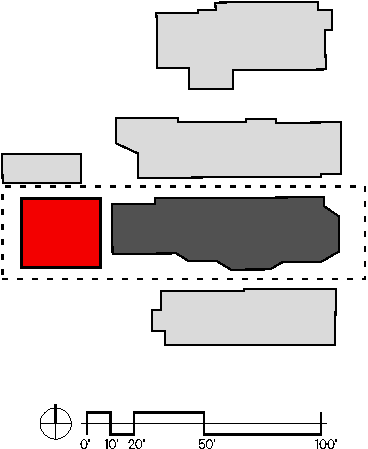
\includegraphics{site1.pdf}
\caption{Site 1: 961 20th Ave, Seattle WA | DADU floor area: 1000 ft$^2$}
\label{site1-plan}
\end{figure}

\begin{figure}[h!]
\centering
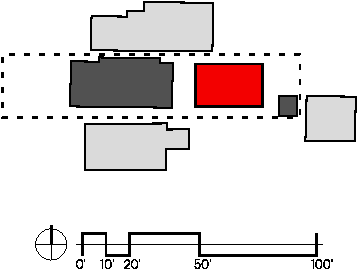
\includegraphics{site2.pdf}
\caption{Site 2: 328 17th Ave, Seattle WA | DADU floor area: 520 ft$^2$}
\label{site2-plan}
\end{figure}

Site selection was primarily driven by orientation between DADU location and existing residences, with each site in a differing neighborhood of Seattle. The Central District, Minor, and Madrona neighborhoods all lie east of downtown Seattle, greatly uphill. Neighborhoods differ slightly in density, street width, and demographics but all chosen sites are within identical SF5000 zoning. Site 1 is located at 961 20th Avenue in the Central District and the DADU is bordered directly by existing structures to the north and east. This DADU is the largest explored, reaching the maximum allowable floor area by single family code\cite{ADUniverseADURules}. Site 2 resides at 328 17th Avenue in Minor and its DADU structure is adjacent to the east of the existing home. This site is unique out of the three, as there is an additional existing structure located on the lot, being a small storage shed to the south-east. Finally, site 3, located at 3413 East Pine Street within Madrona consists of the existing residence facing the street to the north, with DADU location to the south. Neighboring residences to the east and southeast account for the majority of shading effect.

\begin{figure}[h!]
\centering
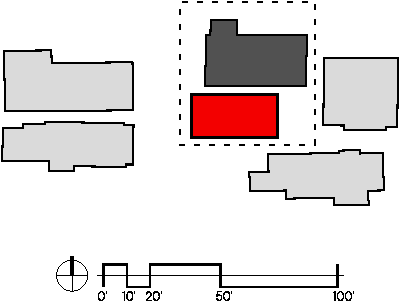
\includegraphics{site3.pdf}
\caption{Site 3: 3413 E Pine St, Seattle WA | DADU floor area: 680 ft$^2$}
\label{site3-plan}
\end{figure}


%TODO Add data visualizations of results
%TODO additional simplified plans or renderings of DADUs and sites
%TODO eui output breakdown and total, point out how only cooling and heating truly vary
%TODO Limitations of Galapagos/Grasshopper workflow

\section{Conclusion}
%TODO Add main conclusion section, user ability to override window sizing and placement- feedback loop?
Looking forward, the intention is to replace the computationally-expensive EnergyPlus simulation with a machine learning model that can predict EUI performance. This technique is essentially  surrogate modeling; that is, a means to approximate/predict the energy performance without doing the thermodynamics calculations required to return a true value. Machine learning algorithms require vast troves of data to learn from in order to increase accuracy past an acceptable threshold. This tool generates the optimized energy simulation data, which in turn becomes the training dataset. Assuming the resultant tool could be hosted on the web, this theoretically increases the rate of adoption by lowering the requirement to utilize the tool. 

\begin{acks}
The author would like to thank Professor Tomas Mendez Echenagucia for his genetic algorithm expertise and input; Teresa Moroseos for her assistance with Honeybee debugging; Professor Alex Anderson and fellow students in the Spring 2021 Arch597 - Research Practicum course at University of Washington for feedback and motivation; Mia Lorentsen for her unending support.
\end{acks}

\begin{funding}
The author(s) received no financial support for the research, authorship, and/or publication of this article.
\end{funding}

\begin{dci}
	The author(s) declared no potential conflicts of interest with respect to the research, authorship, and/or publication of this article.
\end{dci}

\bibliographystyle{SageV}
\bibliography{597_bibliography}

\end{document}
